\documentclass[a4paper]{article}
\usepackage[T1]{fontenc}
\usepackage[utf8]{inputenc}
\usepackage[english]{babel}
\usepackage[hidelinks]{hyperref}
\usepackage{graphicx}
\usepackage{times}
\usepackage{amssymb}
\usepackage{amsmath}
\usepackage{wasysym}
\usepackage{pgfplots}
\pgfplotsset{compat=1.3}
\usepackage{fancyvrb}
\usepackage{enumerate}
\fvset{tabsize=3}
\fvset{fontsize=\small}
\newcommand{\code}{\texttt}

\title{\huge{Performance measurements of a small-space Chromatic Polynomial algorithm}}

\author{Mats Rydberg}
\date{\today}

\begin{document}

\maketitle

\section{Chromatic Polynomial in small space}
The algorithm measured in this performance test is described in Björklund et al \cite{cov_pack}. It is based on the linear-space Fast Zeta Transform described in the same paper, and is proven to perform in time $O(2^n)$ and space $O(1.2916^n)$.

Our input is a graph $G$ on $n$ vertices and $m$ edges. The main subroutine counts the number of ways to colour $G$ using $q$ colours. This is done for $q = 0, 1, \ldots n$, yielding $n + 1$ points $(x_i, y_i)$. These are by definition points which the \emph{chromatic polynomial} $\chi_G(t)$ passes through. $\chi_G(t)$ has exactly degree $n$, and so we have enough information to recover it explicitly using interpolation.

The algorithm in pseudo-code as follows:

\begin{enumerate}[{Step} I.]
 \item \label{q} For $q = 0, 1, \ldots, n$, do
 \begin{enumerate}[1.]
  \item Partition $V$ into $V_1$ and $V_2$.
  \item \label{step1} For each $X_1 \subseteq V_1$, do
  \begin{enumerate}[a)]
   \item \label{indep1} For each independent $Y_1 \subseteq X_1$, do
$$ h[V_2 \setminus N(Y_1)] \leftarrow h[V_2 \setminus N(Y_1)] + z^{|Y_1|} $$
   \item \label{indep2} For each independent $Y_2 \subseteq V_2$, do
$$ l[Y_2] \leftarrow z^{|Y_2|} $$
   \item $h \leftarrow (h\zeta')\cdot l$
   \item $h \leftarrow h\zeta$
   \item For each $X_2 \subseteq V_2$, do
$$ r \leftarrow r + (-1)^{n - |X_1| - |X_2|}\cdot h[X_2]^q $$
  \end{enumerate}
  \item Return coefficient $c_n$ of $z^n$ in $r$.
 \end{enumerate}
 \item Construct interpolating polynomial $\chi_G(t)$ on points $(q, c_{nq})$.
 \item Return $\chi_G(t)$.
\end{enumerate}

$N(Y)$ is the set of all vertices adjacent to at least one vertex in $Y$, $x\zeta'$ denotes the fast up-zeta transform and $x\zeta$ the down-zeta transform (of $x$). $h$ and $l$ are arrays of size $|V_2|$ of polynomials (initialized to containing zeroes), $r$ is a polynomial. For a more detailed description, see \cite{cov_pack}.

\subsection{Optimizations}\label{opts}
%TODO: Extend this text
Graphs for which certain properties can be determined to exist, graph colouring schemes can be greatly improved in terms of performance. %TODO: citation!

\paragraph{Exploiting $q$}
First, we can consider optimizing on the basis of the value of $q$.
\begin{itemize}
\item For $q = 0$, any graph with $n > 0$ can be coloured in 0 ways. For $n = 0$, 0-colouring is undefined. This is a purely semantic question anyway, and empty graphs are not a relevant topic for this paper. This takes $O(1)$ time.
\item For $q = 1$, there are 0 colourings if and only if $|E| > 0$, otherwise there is exactly 1 colouring. This takes $O(n^2)$ time to check, but in practice it is even faster, as we will encounter an edge with high probability before we've scanned the whole graph.
\item For $q = 2$, it is well-known that the graph can be coloured (or found to be non-colourable) in polynomial time using standard techniques (such as breadth-first search). This has not been implemented in my programs.
\end{itemize}

These optimizations will reduce the iterations of the loop at step \ref{q} by three.

\paragraph{Exploiting $w(G)$}
A more sophisticated type of optimization involves exploiting the clique number $\omega(G)$, which is a lower bound of the chromatic number $\chi(G)$\cite{clique}. Knowing that $\omega(G) \geq a$ for some constant $a$ would allow us to immediately skip all steps \ref{q} where $q < a$. In the extreme case of the complete graph $K_n$ (with $\omega(G) = n$) we would skip $n$ evaluations and only run the algorithm for $q = n$, because $K_n$ has no colorings for $q < n$.

Judging from the density of the graph (which is part of the problem input, since $dE = m/m_{max} = \frac{2m}{n(n-1)}$), we can immediately know the \emph{smallest possible} $\omega(G)$. Let us call it $\omega_{min}(G)$. In fact, the following holds:

\begin{equation}\label{omega}
\omega_{min}(G) = \left\{ \begin{array}{lll}
                           n - a & \text{if } m = m_{max} - a & 0 \leq a < \lfloor\frac{n}{2}\rfloor \\
                           \lceil\frac{n}{2}\rceil - a & \text{if } \lfloor(\frac{n}{2})^2\rfloor < m \leq m_{max} - (a + 1)\lfloor\frac{n}{2}\rfloor & 0 \leq a \leq \lfloor\frac{n}{2}\rfloor - 2 \\
                           2 & \text{if } 0 < m \leq \lfloor(\frac{n}{2})^2\rfloor & \\
                           1 & \text{if } m = 0 & \\
                          \end{array}
                  \right.
\end{equation}

As we can see from the equation, only graphs with $m > \lfloor(\frac{n}{2})^2\rfloor$ provides $\omega_{min}(G) > 2$ and for $q \leq 2$ we already have good optimizations. So how dense is a graph where this bound on $m$ holds? Let us specify the threshold density $T_{dE}(n)$ as

$$
T_{dE}(n) = \frac{\lfloor(\frac{n}{2})^2\rfloor}{m_{max}} = 2\frac{\lfloor(\frac{n}{2})^2\rfloor}{n(n-1)} = \left\{ \begin{array}{ll}
          \frac{n}{2(n-1)} & \text{if } n \text{ even}\\
          \frac{n + 1}{2n} = T_{dE}(n+1) & \text{if } n \text{ odd}\\
          \end{array}
  \right.
$$

In conclusion, any graph with $dE > T_{dE}(n)$ can optimize away at least one computation of step \ref{q} above. It also follows that as $n \rightarrow \infty$ we will have $T_{dE}(n) \rightarrow \frac{1}{2}$. The following plot shows how fast we converge for the graphs discussed in this paper.

\begin{center}
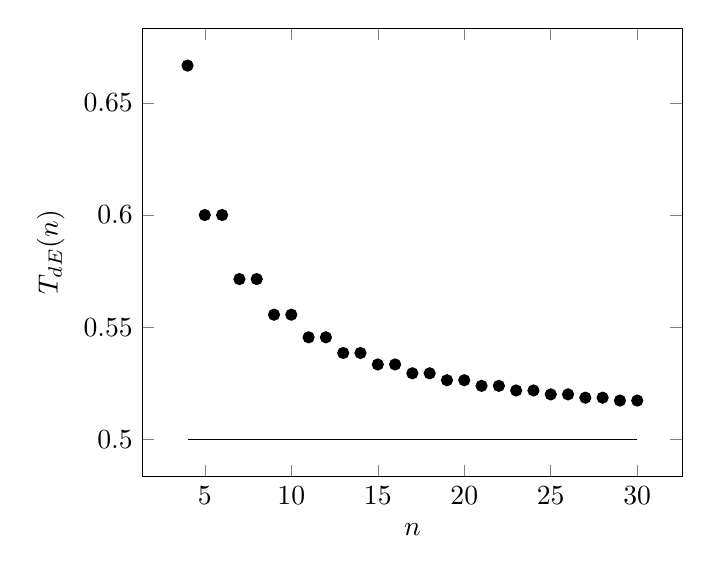
\begin{tikzpicture}
\begin{axis}[%samples at={4,5,6,7,8,9,10,11,12,13,14,...,23},
xlabel=$n$,
ylabel=$T_{dE}(n)$]
%\addplot[black, mark=*, samples=20, domain=4:23] {(2*floor((x/2)^2))/(x*(x-1))};
\addplot[black, only marks, mark=*, samples=14, domain=4:30] {x/(2*(x-1))};
\addplot[black, only marks, mark=*, samples=13, domain=5:29] {(x+1)/(2*x)};
\addplot[black, samples=10, domain=4:30] {1/2};
\end{axis}
\end{tikzpicture}
\end{center}

This result is quite interesting, because for larger graphs, we have a smaller $T_{dE}(n)$, which gives us a higher probability to be able to optimize, and it is also for larger graphs that we are most interested in optimizing techniques. For a graph with $n=23$ and $dE = 75$, we would be able to skip evaluating $q\leq7$, which would yield an expected decrease in time by about 15\%\footnotemark. %TODO update this number 
%UPDATED 1/11 from two tests on pari-0.2 and pari-0.2.1 and graphs 17_80 and 19_85.

\footnotetext{This number is based on experimental results presented below.}

\paragraph{Caching} As we will see below, in comparison to another algorithm for finding $\chi_G(t)$ (actually for finding the Tutte polynomial, but this encodes $\chi_G$ as well), we are using not just less space, but \emph{much} less space. This tempts the thought of being able to do some kind of caching technique, to trade off space for time. No certain structure for a caching scheme has been invented yet, however.

\paragraph{Parallelization} Most importantly, and also mentioned in \cite{cov_pack}, is to parallelize computations of step \ref{step1}, as these are independent of eachother. This would yield significant time improvements in theory. With access $2^{|V_1|}$ processors, we would be able to execute the program in time $O(1.5486^n)$. Typically, we will only have access to a constant number of processors in practice, allowing each of them to execute a range of iterations of step \ref{step1}. As presented below, we can expect to reduce the time consumption of the program by a factor of around 4. %TODO: make sure this number is correct.

We may also parallelize the steps \ref{q} on $O(n)$ parallel CPUs. This would not reduce the exponential factor of the time complexity, but it does reduce the polynomial factor and it is likely to give significant results in practice. I do not investigate this optimization technique, as my resources are already exhausted by parallelizing step \ref{step1}.

\section{Implementation details}
My test implementation only partially supports values of $n$ over 64. In practice, the program does not perform very well for such large problems anyway, so for the meantime this restriction is not critical. It also allows me to use a quite natural way of encoding sets by simply letting them be a whole integer word, 64 bits long. A one in position $i$ of the word means that vertex $i$ in the graph is present in the set represented by the word.

I've chosen to support adjacency matrices as input structure, representing an arbitrary graph\footnotemark. Another common graph representation is the edge list, which is faster, but since our problem is exponentially hard, another degree of a polynomial term doesn't really affect our performance very much. It is also more straight-forward for me to generate randomized graphs using an adjacency matrix.

\footnotetext{Multiple edges and self-edges are two graph invariants that often need special treatment in graph-based algorithms. This is not the case for graph colouring. Any self-edge means the graph is not colourable (a vertex would need to have a different colour from itself), so these are naturally not allowed. In my implementation, I assume they do not exist. Any multiple edge doesn't affect the problem at all, as we are merely considering the \emph{existence} of an edge between two vertices; if there are more than one that doesn't matter.}

%TODO: Write own polynomial? If not, delete this part.

For polynomial representation, I've implemented two libraries for number theoretic calculations to be used by my program. These also provide interpolation functionality. For reference, I've also supplied my own implementation of a polynomial, to measure how much the choice of polynomial implementation actually influences the overall performance of the program. Unwilling to implement also my own interpolation functionality, I've decided to use NTL's interpolation implementation. The interpolation step is not critical to performance, so this choice is pretty much arbitrary.

%TODO: Investigate also FLINT?

\subsection{NTL 6.0.0}
The first is NTL, Number Theoretic Library, written in C++ by Victor Shoup at New York University\cite{ntl}. It is advertised as one of the fastest implementations of polynomial arithmetic, which is all that I am interested in. Unfortunately, it does not provide any non-trivial way of exponentiating polynomials, and its multiplication algorithms are a bit lackluster after some careful studying. It is very easy to use, provides its own garbage collection and has a rich, high-level interface for library usage.

The functions I use are primarily these: 

\begin{itemize}
 \item \code{ZZX.operator+=()}
 \subitem Addition and assignment for polynomials. %TODO Documentation citation
 \item \code{ZZX.operator*=()}
 \subitem Multiplication and assignment for polynomials. %TODO Doc citation
\end{itemize}

Binaries are called \code{bhkk-ntl-x.y.z}.

\subsection{PARI 2.5.5}
Experiencing the relative lack of performance boost from the NTL implementation led me to find also the PARI project. It is written in C mainly by a group of French computer scientists at Université Bordeaux \cite{pari}, together with a calculator-like interface (\code{gp}) to be used by an end-user (comparable to Maple). The PARI library is provided at a much lower level, requires the user to garbage collect (since it is written in C, after all), has a much steeper learning curve and a very detailed but hard-to-grasp documentation. It is a bit unclear to me how exactly PARI implements polynomial exponentiation and multiplication, but from the impression I've got and, more importantly, its performance, it has to be non-trivial.

The functions I use are primarily these: 

\begin{itemize}
 \item \code{ZX\_add()}
 \subitem Addition for polynomials. %TODO: doc citation
 \item \code{ZX\_mul()}
 \subitem Multiplication for polynomials. %TODO: citation from documentation
 \item \code{gpowgs()}
 \subitem General exponentiation for PARI types. Used for polynomials.
\end{itemize}

Binaries are called \code{bhkk-pari-x.y.z}.


%TODO: is this part necessary?
%The PARI library implements its own stack, which it needs to have allocated before any function calls can be made. Preferably, a large enough stack should be allocated at the start of the program, so that re-allocations will not be necessary. I am allocating 50MB of memory for the stack, which is more than enough for most instances. This has a side effect in the measurements of memory usage, meaning that the virtual memory peak is constant for all PARI executions.

\subsection{GMP 5.1.2}
Both the libraries I use to represent polynomials allow (and encourage) the user to configure them using GMP\cite{gmp} as the low-level interface for integral arithmetic (actually, for all arithmetic, but I only use integers). Authors of both libraries suggest that using GMP instead of their own, native low-level interface will yield significant performance boosts. For this reason, I have done just that. GMP is well documented, easy-to-use, provides both C and C++ interfaces and even has a well-maintained bug reporting facility (I got an answer the same day!). GMP allows the user a rich variety of configuration options, and I've tried to optimize as narrowly as possible to get maximum performance on one machine.

In my implementation, I only use GMP to generate randomized graphs. All arithmetic is performed via the interfaces of PARI and NTL, which themselves call underlying GMP functions. My own naive implementation of polynomials also uses GMP types directly.

\section{Algorithm performance parameters}
The algorithm has some perks that make it perform better or worse for different input. In this section I aim to explore a few of these characteristics.

\subsection{Sparse and dense graphs}\label{sparsedense}
The algorithm in itself is designed in a way that allow for a smaller degree of complexity for \emph{dense} graphs. This is in contrast to many of the algorithms which I've studied for the graph colouring problem. And this is not only for very dense graphs, but performance is in fact a function that is directly related to graph density, and consistently performs better for every additional edge to a graph. This follows directly from steps \ref{indep1} and \ref{indep2} above:

$$ h[V_2 \setminus N(Y_1)] \leftarrow h[V_2 \setminus N(Y_1)] + z^{|Y_1|} $$

$$ l[Y_2] \leftarrow z^{|Y_2|} $$

Recall that these lines will only be executed for \emph{independent} sets $Y_1$ and $Y_2$. As graph density increases, fewer subsets of the vertex set $V$ will be independent, and less of these lines will be executed. This has a direct effect in reducing some additions and assignments, but more importantly has side effects in all subsequent steps. Addition-assignment with zero is a non-operation. Multiplication with zero is trivial, and yields even more zeroes. In the extreme case of a complete graph $G=(V,E)$, where all independent subsets of $V$ are of size 1, the most time-critical operation may be the independence testing function (which is executed on all subsets regardless of $G$).

This discussion of course also applies to a \emph{sparse} graph, in which case we will have \emph{fewer} zeroes and more non-trivial operations.

\subsection{Multiplication algorithms}
%TODO: Count number of multiplications/additions/powerings
Much of the complexity of the whole algorithm comes down to how polynomial multiplication is performed. The most common operation is to multiply two polynomials of \emph{small} degree but with \emph{large} coefficients. This is because the degree of the polynomials increase as $O(n)$ while their coefficients increase as $O(2^n)$. %TODO: Citation?

Trivially, a polynomial multiplication would be to expand over both operands' coefficients and cross-multiply them in a standard fashion. This is very inefficient, and many techniques have been developed to deal with this problem. In fact, the original issue has always been to multiply two large integers, but the most sophisticated results show methods that make use of polynomials for this purpose. The algorithm with the best asymptotic complexity is the Schönhage-Strassen algorithm \cite{strass}, but it has a large overhead and becomes useful only for huge operands. It is based on a Fast Fourier Transform. The most go-to algorithm seems to be the Toom-Cook \cite{toom-cook} (aka Toom-$k$) family, in which Toom-2 (aka Karatsuba) or Toom-3 are the most common.

The technique used in Toom-$k$ for multiplying two large integers is to split them up in parts, introduce a polynomial representation of degree $k-1$ for these parts (the parts are coefficients), evaluate the polynomials at certain points (the choice of points is critical%TODO: citation!
), perform pointwise multiplication of the evaluated polynomials, interpolate the resulting points into a resulting polynomial, and finally reconstruct the integer from the coefficients of the resulting polynomial. This technique is easily translated for polynomial multiplication as well, where the first and last steps would be skipped.

The GMP library supports Karatsuba, Toom-3, Toom-4, Toom-6.5, Toom-8.5 and Schönhage-Strassen \cite[p 90]{gmp}, which means all libraries used in my programs uses these algorithms \emph{at least} when multiplying integers (ie, coefficients of polynomials).

NTL implements Karatsuba, Schönhage-Strassen and another FFT-based technique for polynomials \cite{ntl_zzx}.

I have not found any documentation specifying which algorithms are implemented in the PARI library for polynomial multiplication. From analyzing the source code, it seems as if PARI ''converts'' the polynomial to an integer and submits it to its integer multiplication function (which would be one of GMPs).

\section{Experimental results}
My tests are performed on randomized graphs, generated for some values of $n$ and $dE$. The algorithm does not assume anything about the general structure of the graphs, and only exploits the graph invariants mentioned in \ref{opts}.

%Here follows the performance graphs for all tests. Some interpretational text is also provided. The blue circles show user time in the time graphs and virtual memory in the memory graphs. The red squares show system time in the time graphs and resident set size in the memory graphs.

The following instances have been executed:

\begin{itemize}
 \item Increasing $n$ in interval $[4, 23]$.
 \subitem ''Dense'' graphs, $dE = 75$.
 \subitem ''Sparse'' graphs, $dE = 40$.
 \item Increasing density, $n = 19$, $dE \in [5, 100]$.
 \item ''Large'' instances, $n = 25$ and $n = 30$, $dE = 75$.
 \subitem This is only done for the fastest implementation.
 \item Evaluation step, $q = 2, 3, \ldots, 19$, $n = 19$, $dE = 40$.
 %\subitem This is not done for the naive implementation.
\end{itemize}

The program has evolved through the development process as new optimizations have been implemented. In order to measure the effects of each optimization simulations have been run on a number of different versions of the programs. In an effort to provide completeness while at the same time not flood this paper with graphs, I've tried to structure up this section by specifying some identifiers for the executables that have been run in simulations.

Due to the linearity of the development process, each executable implements all optimizations included in the ones above them (where applicable).

\begin{tabular}{c|c|c|c}
 Identifier & Attributes & Polynomial library & Version number \\ \hline
 \code{aka} & Base & PARI & 0.1 \\
 \code{senko} & Base & NTL & 0.1 \\
 \code{midori} & Parallelization & PARI & 0.2 \\
 \code{kimidori} & Parallelization & NTL & 0.2 \\
 \code{buryu} & Min-max clique number & PARI & 0.3-beta \\
 \code{mizudori} & Min-max clique number & NTL & 0.3-beta \\
\end{tabular}

% prasinus, -a, - um. green
% purpureus, -a, -um. purple (purple)
% caeruleus, -a, -um. blue (caerulean)
% lividus, -a, -um. black and blue (livid)
% niger. black (denigrate)
% ater, atra, atrum. black (dark) (atrabilious)
% fuscus, -a, -um. dark (obfuscate)
% ravus, -a, -um. gray
% canus, -a, -um. gray or white (hair)
% albus, -a, -um. white (alb)
% flavus, -a, -um. yellow (pale) (riboflavin)
% fulvus, -a, -um. golden yellow
% croceus, -a, -um. saffron (crocus)
% ruber, rubra, rubrum. red (rubella)

\subsection{Measurements}
All tests are performed on the same machine, with the following specifications.

\begin{center}
\begin{tabular}{|c|c|} \hline
CPU (cores, threads) & Intel i7-3930K 3.2GHz (6, 12) \\ \hline
OS & GNU/Linux 3.8.13.4-desktop-1.mga3 (Mageia 3) x86\_64 \\ \hline
Memory & 16GB DDR3 1333Mhz \\ \hline
Compilator & GCC 4.7.2 (g++) \\ \hline
\end{tabular}
\end{center}

For all time and memory measurements, the GNU time 1.7 program is used \cite{time}. The user time, elapsed time (real time) and peak resident set size are the data points recovered as measurements.

% Data is collected by pausing the process just before normal termination and reading from the process' stat file in \code{/proc/[pid]/stat} for time and \code{/proc/[pid]/status} for memory peaks (see the linux man pages for \code{proc} \cite{proc}). 
% %TODO: Make sure this is correct
% The information gathered is the amount of time used (both user and system time), the peak size of the resident set and the peak virtual memory.
% 
% This measuring process is not applicable for third party software, so in my comparisons to the Haggard-Pearce algorithm \cite{haggard}, I've used the GNU \code{time} program (version 1.7). Time data is much the same between both methods, but memory usage data is not.

\subsubsection{What is space?}\label{whatisspace}
%TODO: Write something about how space and memory relate to eachother.

\subsection{PARI 2.5.5}
Some text about PARI. %TODO

\subsubsection{Increasing $n$}

This is time as a function of $n$. Expected function in theory is $O^*(2^n)$.

\begin{center}
\begin{tabular}{rl}
\begin{tikzpicture}
\begin{axis}[legend pos=north west,baseline,trim axis left,small,
xlabel=$n$,
ylabel=CPU time (ms)]
\addplot table[x=n,y=ut] {../output/javatests/pari_all1};
\addplot[red,mark=triangle*] table[x=n,y=ut] {../output/javatests/pari_all2};
\addplot[black,mark=diamond*] table[x=n,y=ut] {../output/parsed_results/chr_pol_pari_pari_pll_time1};
\legend{Dense, Sparse, 2nd method}
%\addplot table[x=n,y=tt] {../output/parsed_results/chr_pol_ntl_ntl_all_time1};
\end{axis}
\end{tikzpicture}
&
\begin{tikzpicture}
\begin{axis}[legend pos=north west,baseline,trim axis right,small,
xlabel=$n$,
ylabel=Real time (ms), yticklabel pos=right, ylabel style={align=right}]
\addplot table[x=n,y=rt] {../output/javatests/pari_all1};
\addplot[red,mark=triangle*] table[x=n,y=rt] {../output/javatests/pari_all2};
\legend{Dense, Sparse}
%\addplot table[x=n,y=tt] {../output/parsed_results/chr_pol_ntl_ntl_all_time1};
\end{axis}
\end{tikzpicture}
% \\
% \begin{tikzpicture}
% \begin{axis}[legend pos=north west,baseline,trim axis left,small,title=Dense graphs,
% xlabel=$n$,
% ylabel=Time (ms)]
% \addplot table[x=n,y=ut] {../output/javatests/pari_all1};
% \addplot[red,mark=triangle*] table[x=n,y=rt] {../output/javatests/pari_all1};
% \legend{CPU time, Real time}
% %\addplot table[x=n,y=tt] {../output/parsed_results/chr_pol_ntl_ntl_all_time1};
% \end{axis}
% \end{tikzpicture}
% &
% \begin{tikzpicture}
% \begin{axis}[legend pos=north west,baseline,trim axis right,small,
% xlabel=$n$,
% ylabel=Real time (ms), yticklabel pos=right, ylabel style={align=right}]
% \addplot table[x=n,y=rt] {../output/javatests/pari_all1};
% \addplot[red,mark=triangle*] table[x=n,y=rt] {../output/javatests/pari_all2};
% \legend{dense, sparse}
% %\addplot table[x=n,y=tt] {../output/parsed_results/chr_pol_ntl_ntl_all_time1};
% \end{axis}
% \end{tikzpicture}
\\
\end{tabular}
\end{center}

Here we have memory usage as a function of $n$. Expected function from theory is $O^*(1.2916^n)$.

\begin{center}
\begin{tabular}{c}
\begin{tikzpicture}
\begin{axis}[legend pos=north west,baseline,trim axis left,small,
xlabel=$n$,
ylabel=Peak resident set size (kB)]
\addplot table[x=n,y=rss] {../output/javatests/pari_all1};
\addplot[red,mark=triangle*] table[x=n,y=rss] {../output/javatests/pari_all2};
\legend{Dense, Sparse}
%\addplot table[x=n,y=tt] {../output/parsed_results/chr_pol_ntl_ntl_all_time1};
\end{axis}
\end{tikzpicture}
% &
% \begin{tikzpicture}
% \begin{axis}[legend pos=north west,baseline,trim axis right,small,
% xlabel=$n$,
% ylabel=Peak resident set (kB), yticklabel pos=right, ylabel style={align=right}]
% \addplot table[x=n,y=rss] {../output/javatests/pari_all1};
% \addplot[red,mark=triangle*] table[x=n,y=rss] {../output/javatests/pari_all2};
% \legend{Dense, Sparse}
% %\addplot table[x=n,y=tt] {../output/parsed_results/chr_pol_ntl_ntl_all_time1};
% \end{axis}
% \end{tikzpicture}
\\
\end{tabular}
\end{center}


\subsubsection{Parallelization}
Here we investigate how our parallelization scheme acts as we increase the number of threads. We plot the function of user and real time as we increase the number of threads. Recall that our maximum \emph{actual} parallelization width is 12.

\begin{center}
\begin{tabular}{rl}
\begin{tikzpicture}
\begin{axis}[legend pos=south east,trim axis left,small,
xlabel=\# threads,
ylabel=CPU time (ms)]
\addplot[blue, mark=|] table[x=t,y=ut] {../output/javatests/pari_all3};
\addplot[red, mark=-] table[x=t,y=ut] {../output/javatests/pari_all4};
\legend{Dense, Sparse}
%\addplot table[x=n,y=tt] {../output/parsed_results/chr_pol_ntl_ntl_all_time1};
\end{axis}
\end{tikzpicture}
&
\begin{tikzpicture}
\begin{axis}[legend pos=north east,trim axis right,small,
xlabel=\# threads,
ylabel=Real time (ms), yticklabel pos=right, ylabel style={align=right}]
\addplot[blue, mark=|] table[x=t,y=rt] {../output/javatests/pari_all3};
\addplot[red,mark=-] table[x=t,y=rt] {../output/javatests/pari_all4};
\legend{Dense, Sparse}
%\addplot table[x=n,y=tt] {../output/parsed_results/chr_pol_ntl_ntl_all_time1};
\end{axis}
\end{tikzpicture}
\\
\end{tabular}
\end{center}

There seem to be no notable difference in how sparse and dense graphs parallelize. As expected, the plots peak at 12 threads. What is not expected is that the top performance was measured for 45 threads. It is not easy to realize that some threads will terminate much sooner than others (because they happened to get a range of subsets which were more frequently independent, see section \ref{sparsedense}), and so using > 12 threads could be useful. It is unclear why 45 is the best (measured) value, however.

Another interesting note to take is that for 100 threads, the gain in processing dense versus sparse graphs has disappeared. This can partly be explained by the fact that the OS is now spending lots of time context switching the 100 threads over the 12 CPUs, but from a more algorithmic point of view, we can make another argument. As we let each thread iterate over fewer and fewer subsets from step \ref{step1}, our real time consumption is more and more dominated by the one thread that takes the longest time to execute. That is, the thread that was allocated with the ''worst'' range of subsets. ''Bad'' ranges are more common when the graph is sparse, but as we divide the subsets into smaller ranges, the ''worst'' range decreases in ''badness'' faster for the sparse graphs than for the dense. It would seem that they have more or less converged for the graph above at 100 threads.

\bigskip

Here we compare CPU time to real time consumption and also to the CPU time used by the single threaded version, and get an indication of how powerful our parallelization is to performance. %TODO: How does this discussion relate to the one in previous paragraphs? check this up and make a complete and composite discussion.

\begin{center}
\begin{tabular}{c}
\begin{tikzpicture}
\begin{axis}[legend pos=north west,baseline,trim axis left,title=Dense graphs,
xlabel=$n$,
ylabel=Time (ms)]
\addplot table[x=n,y=ut] {../output/javatests/pari_all1};
\addplot[red,mark=triangle*] table[x=n,y=rt] {../output/javatests/pari_all1};
\addplot[black,mark=diamond*] table[x=n,y=ut] {../output/parsed_results/chr_pol_pari_pari_all_time1};
%\addplot[magenta] table[x=n,y expr=\thisrow{ut}/12] {../output/javatests/pari_all1};
\legend{CPU time, Real time, Single thread}
\end{axis}
\end{tikzpicture}
\\
\end{tabular}
\end{center}

\begin{center}
\begin{tabular}{rl}
\begin{tikzpicture}
\begin{axis}[legend pos=south east,baseline,trim axis left,small,
xlabel=Threads,
ylabel=Time (ms)]
\addplot table[x=n,y=ut] {../output/parsed_results/chr_pol_pari_pari_pll_time1};
\addplot[red,mark=triangle*] table[x=n,y=ut] {../output/parsed_results/chr_pol_pari_pari_pll_time2};
\legend{dense, sparse}
%\addplot table[x=n,y=tt] {../output/parsed_results/chr_pol_ntl_ntl_all_time1};
\end{axis}
\end{tikzpicture}
&
\begin{tikzpicture}
\begin{axis}[legend pos=north east,baseline,trim axis right,small,
xlabel=Threads,
ylabel=Weighted time (ms), yticklabel pos=right, ylabel style={align=right}]
\addplot table[x=n,y expr=\thisrow{ut}/x] {../output/parsed_results/chr_pol_pari_pari_pll_time1};
\addplot[red,mark=triangle*] table[x=n,y expr=\thisrow{ut}/x] {../output/parsed_results/chr_pol_pari_pari_pll_time2};
\legend{dense, sparse}
%\addplot table[x=n,y=tt] {../output/parsed_results/chr_pol_ntl_ntl_all_time1};
\end{axis}
\end{tikzpicture}\\
\end{tabular}
\end{center}

\begin{center}
\begin{tikzpicture}
\begin{axis}[legend pos=south east,
xlabel=Threads,
ylabel=Resident Set Size (kB)]
\addplot table[x=n,y=rss] {../output/parsed_results/chr_pol_pari_pari_pll_mem1};
\addplot[red,mark=triangle*] table[x=n,y=rss] {../output/parsed_results/chr_pol_pari_pari_pll_mem2};
\legend{dense, sparse}
%\addplot table[x=n,y=tt] {../output/parsed_results/chr_pol_ntl_ntl_all_time1};
\end{axis}
\end{tikzpicture}
\end{center}

\begin{center}
\begin{tikzpicture}
\begin{axis}[legend pos=north east,
xlabel=\# threads,
ylabel=Weighted Resident Set Size (kB)]
\addplot table[x=n,y expr=\thisrow{rss}/x] {../output/parsed_results/chr_pol_pari_pari_pll_mem1};
\addplot[red,mark=triangle*] table[x=n,y expr=\thisrow{rss}/x] {../output/parsed_results/chr_pol_pari_pari_pll_mem2};
\legend{dense, sparse}
%\addplot table[x=n,y=tt] {../output/parsed_results/chr_pol_ntl_ntl_all_time1};
\end{axis}
\end{tikzpicture}
\end{center}

% \subsubsection{''Dense'' graphs}
% \begin{center}
% \begin{tikzpicture}
% \begin{axis}[
% xlabel=$n$,
% ylabel=Time (ms)]
% \addplot table[x=n,y=ut] {../output/parsed_results/chr_pol_pari_pari_all_time1};
% %\addplot table[x=n,y=st] {../output/parsed_results/chr_pol_pari_pari_all_time1};
% %\addplot table[x=n,y=tt] {../output/parsed_results/chr_pol_pari_chr_pol1_time1};
% \end{axis}
% \end{tikzpicture}
% \end{center}
% 
% Time usage shows us what we expect; a strong, sudden increase as $n$ grows. At $n=15$, execution exceeds 1 second. At $n=21$ we are over 200 seconds, and at $n=23$ execution takes over 1000 seconds.
% 
% Is this increase exponential? For reference, let us assume that each accounted operation takes 0.1 milliseconds. Since our time complexity in terms of operations increase as $O(2^n)$, we can plot this as $f_t(x) = \frac{1}{10}2^x$.
% 
% \begin{center}
% \begin{tikzpicture}
% \begin{axis}[legend pos=north west,
% xlabel=$n$,
% ylabel=Time (ms)]
% \addplot[blue, mark=*] table[x=n,y=ut] {../output/parsed_results/chr_pol_pari_pari_all_time1};
% \addlegendentry{measured time}
% \addplot[red,mark=triangle*,domain=4:23] {(1/10)*2^x};
% \addlegendentry{expected time ($f_t$)}
% %\addplot table[x=n,y=st] {../output/parsed_results/chr_pol_pari_pari_all_time1};
% %\addplot table[x=n,y=tt] {../output/parsed_results/chr_pol_pari_chr_pol1_time1};
% \end{axis}
% \end{tikzpicture}
% \end{center}
% 
% From this comparison, we may conclude that time consumption of the program is no better than $O(2^n)$, given above assumptions.
% 
% \begin{center}
% \begin{tikzpicture}
% \begin{axis}[legend pos=north west,
% xlabel=$n$,
% ylabel=Resident set size (kB)]
% \addplot table[x=n,y=rss] {../output/parsed_results/chr_pol_pari_pari_all_mem1};
% \addplot[red, mark=triangle*,domain=4:23] {(4)*(1.2916)^x + 2600};
% \legend{measured memory, theoretical space ($f_m$)}
% %\addplot table[x=x,y=2exp] {../misc/functables/129exp};
% %\addplot table[x=n,y=vm] {../output/parsed_results/chr_pol_pari_pari_all_mem1};
% \end{axis}
% \end{tikzpicture}
% \end{center}
% 
% Assuming one unit of ''space'' (see section \ref{whatisspace}) takes about 4KB of memory, we can estimate the expected memory usage as $f_m(x) = 4\cdot1.2916^n + c$, where $c$ is our constant overhead, where we find $c = 2600$ is coherent with experimental results. $f_m$ grows as $O(1.2916^n)$, which is the specified space consumption from \cite{cov_pack}.

% \subsubsection{''Sparse'' graphs}
% 
% \begin{center}
% \begin{tikzpicture}
% \begin{axis}[
% xlabel=$n$,
% ylabel=time (ms)]
% \addplot table[x=n,y=ut] {../output/parsed_results/chr_pol_pari_pari_all_time2};
% %\addplot table[x=n,y=st] {../output/parsed_results/chr_pol_pari_pari_all_time2};
% %\addplot table[x=n,y=tt] {../output/parsed_results/chr_pol_pari_chr_pol1_time2};
% \end{axis}
% \end{tikzpicture}
% \end{center}
% A typical exponentially increasing time curve.
% 
% \begin{center}
% \begin{tikzpicture}
% \begin{axis}[
% xlabel=$n$,
% ylabel=Resident set size (MB)]
% \addplot table[x=n,y=rss] {../output/parsed_results/chr_pol_pari_pari_all_mem2};
% %\addplot table[x=n,y=vm] {../output/parsed_results/chr_pol_pari_pari_all_mem2};
% \end{axis}
% \end{tikzpicture}
% \end{center}
% More or less constant resident set size. Some inaccuracy in the measuring process can be suspected, but the ''jump'' is not as large as it seems.

% \subsubsection{Comparing ''sparse'' and ''dense''}
% As we discussed in section \ref{sparsedense}, the algorithm performs better on dense graphs. But how much better?
% 
% \begin{center}
% \begin{tikzpicture}
% \begin{axis}[legend pos=north west,
% xlabel=$n$,
% ylabel=Time (ms)]
% \addplot[red, mark=o] table[x=n,y=ut] {../output/parsed_results/chr_pol_pari_pari_all_time1};
% \addplot[blue,mark=o] table[x=n,y=ut] {../output/parsed_results/chr_pol_pari_pari_all_time2};
% \addplot[black,domain=4:23] {(1/10)*2^x};
% \legend{dense, sparse, $f_t$}
% \end{axis}
% \end{tikzpicture}
% \end{center}
% 
% We have a clear difference. At the largest measured $n = 23$, a graph with almost twice as many edges does the job in about half the time.
% 
% \begin{center}
% \begin{tikzpicture}
% \begin{axis}[legend pos=north west,
% xlabel=$n$,
% ylabel=Resident set size (kB)]
% \addplot[red, mark=o] table[x=n,y=rss] {../output/parsed_results/chr_pol_pari_pari_all_mem1};
% \addplot[blue, mark=o] table[x=n,y=rss] {../output/parsed_results/chr_pol_pari_pari_all_mem2};
% \addplot[black,domain=4:23] {(4)*(1.2916)^x + 2600};
% \legend{dense, sparse, $f_m$}
% \end{axis}
% \end{tikzpicture}
% \end{center}
% 
% And of course the sparse graphs use more space as well, implicated by the same conclusions. 

\subsubsection{Increasing density}
So, we've seen that the density of the graph is important to the performance of the algorithm. But how much falloff can we expect? And are there any certain points of extra interest?

\begin{center}
\begin{tabular}{rl}
\begin{tikzpicture}
\begin{axis}[legend pos=north east,trim axis left,small,
xlabel=$dE$,
ylabel=Time (ms)]
%\addplot[blue, mark=*] table[x=dE,y=ut] {../output/javatests/pari_all6};
\addplot[blue, mark=*] table[x=dE,y=rt] {../output/javatests/pari_all6};
\legend{Real time}
\end{axis}
\end{tikzpicture}
&
\begin{tikzpicture}
\begin{axis}[legend pos=north east,trim axis right,small, yticklabel pos=right, ylabel style={align=right},
xlabel=$dE$,
ylabel=Time (ms)]
\addplot[blue, mark=*] table[x=dE,y=rt] {../output/javatests/pari_all6};
\addplot[red, mark=triangle*] table[x=dE,y=ut] {../output/javatests/pari_all6};
\legend{Real time, CPU time}
\end{axis}
\end{tikzpicture}
\\
\begin{tikzpicture}
\begin{axis}[legend pos=north east,trim axis left,small,
xlabel=$dE$,
ylabel=CPU time (ms)]
\addplot[blue, mark=*] table[x=df,y=ut] {../output/parsed_results/chr_pol_pari_pari_all_time3};
\addplot[red, mark=triangle*] table[x=dE,y=ut] {../output/javatests/pari_all6};
\legend{Single thread, Parallelized}
\end{axis}
\end{tikzpicture}
&
\begin{tikzpicture}
\begin{axis}[legend pos=north east,trim axis right,small, yticklabel pos=right, ylabel style={align=right},
xlabel=$dE$,
ylabel=Time (ms)]
\addplot[blue, mark=*] table[x=df,y=ut] {../output/parsed_results/chr_pol_pari_pari_all_time3};
\addplot[red, mark=triangle*] table[x=dE,y=rt] {../output/javatests/pari_all6};
\legend{Single thread, Real time}
\end{axis}
\end{tikzpicture}
\\
\end{tabular}
\end{center}

The time falloff follows the same pattern in user time and in real time. The pattern is also the same if we compare to the single thread version.


Memory as a function of density:

\begin{center}
\begin{tabular}{rl}
\begin{tikzpicture}
\begin{axis}[legend pos=north east,trim axis left,small,
xlabel=$dE$,
ylabel=Peak resident set size (kB)]
\addplot[blue, mark=*] table[x=dE,y=rss] {../output/javatests/pari_all6};
%\legend{Real time}
\end{axis}
\end{tikzpicture}
&
\begin{tikzpicture}
\begin{axis}[legend pos=north east,trim axis right,small, yticklabel pos=right, ylabel style={align=right},
xlabel=$dE$,
ylabel=Peak resident set size (kB)]
\addplot[blue, mark=*] table[x=dE,y=rss] {../output/javatests/pari_all6};
\addplot[red, mark=triangle*] table[x=df,y=rss] {../output/parsed_results/chr_pol_pari_pari_all_mem3};
\legend{Parallelized, Single thread}
\end{axis}
\end{tikzpicture}
\\
\end{tabular}
\end{center}

Single threaded version:

\begin{center}
\begin{tikzpicture}
\begin{axis}[
xlabel=$dE$,
ylabel=Time (ms)]
\addplot table[x=df,y=ut] {../output/parsed_results/chr_pol_pari_pari_all_time3};
%\addplot[black, domain=5:100] {1/((0.05)*x)*7*10^4};
%\addplot[black, domain=5:100] {1.5*10^5 - 1350*x};
%\addplot table[x=df,y=st] {../output/parsed_results/chr_pol_pari_pari_all_time3};
%\addplot table[x=n,y=tt] {../output/parsed_results/chr_pol_pari_chr_pol1_time3};
\end{axis}
\end{tikzpicture}
\end{center}

\begin{center}
\begin{tikzpicture}
\begin{axis}[
xlabel=$dE$,
ylabel=Resident set size (kB)]
\addplot table[x=df,y=rss] {../output/parsed_results/chr_pol_pari_pari_all_mem3};
%\addplot table[x=df,y=vm] {../output/parsed_results/chr_pol_pari_pari_all_mem3};
\end{axis}
\end{tikzpicture}
\end{center}

As we can see, both time and space consumption falls off the most as we add the first edges. At 20\% density we use 30\% less space and over 40\% less time as compared to 5\% density. Our best performance is on complete graphs, even though we do not implement any ''special treatment'' for graphs of certain density.

\subsubsection{''Large'' instance}
Single thread: (gets beat) on m\_25\_40 (I think!) %TODO 40 or 75?
\begin{center}
 \begin{tabular}{|c|c|c|} \hline
  Program & Time (s) & Peak resident set size (MB) \\ \hline
  \code{chr\_pol\_pari} & 10870 & 33.93 \\ \hline
  \code{tutte} & 4906 & 20129.5 \\ \hline
 \end{tabular}

\end{center}

12 threads: (pwns) on m\_30\_75

\begin{center}
 \begin{tabular}{|c|c|c|c|} \hline
  Program & CU time (s) & Real time (s) & Peak resident set size (MB) \\ \hline
  \code{chr\_pol\_pari} & 559,841 & 49,651 & 2,584 \\ \hline
  \code{tutte} & > 94,000 & > 95,000 & 40,135 \\ \hline
 \end{tabular}

\end{center}

\code{tutte} did not finish and was stopped after 95,000 seconds (over 26 hours).


% PARI:
% Command being timed: "bins/chr_pol_pari input/adjm/m_25_40"
%         User time (seconds): 10870.95
%         System time (seconds): 1.98
%         Percent of CPU this job got: 75%
%         Elapsed (wall clock) time (h:mm:ss or m:ss): 4:00:29
%         Average shared text size (kbytes): 0
%         Average unshared data size (kbytes): 0
%         Average stack size (kbytes): 0
%         Average total size (kbytes): 0
%         Maximum resident set size (kbytes): 34752
%         Average resident set size (kbytes): 0
%         Major (requiring I/O) page faults: 0
%         Minor (reclaiming a frame) page faults: 2281
%         Voluntary context switches: 2
%         Involuntary context switches: 20348
%         Swaps: 0
%         File system inputs: 0
%         File system outputs: 0
%         Socket messages sent: 0
%         Socket messages received: 0
%         Signals delivered: 0
%         Page size (bytes): 4096
%         Exit status: 0

% Haggard:
%Command being timed: "./tutte --chromatic -c5000M /home/sx/repo/xjobb/head/common/input/edgelists/el_25_120"
% User time (seconds): 4906.30
%         System time (seconds): 70.75
%         Percent of CPU this job got: 99%
%         Elapsed (wall clock) time (h:mm:ss or m:ss): 1:22:57
%         Average shared text size (kbytes): 0
%         Average unshared data size (kbytes): 0
%         Average stack size (kbytes): 0
%         Average total size (kbytes): 0
%         Maximum resident set size (kbytes): 20612608
%         Average resident set size (kbytes): 0
%         Major (requiring I/O) page faults: 0
%         Minor (reclaiming a frame) page faults: 1288424
%         Voluntary context switches: 1
%         Involuntary context switches: 14932
%         Swaps: 0
%         File system inputs: 0
%         File system outputs: 0
%         Socket messages sent: 0
%         Socket messages received: 0
%         Signals delivered: 0
%         Page size (bytes): 4096
%         Exit status: 0

\subsubsection{Evaluation step}

% 
% \subsubsection{Test 1}
% \vspace{3mm}
% \begin{center}
% \begin{tikzpicture}
% \begin{axis}[
% xlabel=$n$,
% ylabel=time (ms)]
% \addplot table[x=n,y=ut] {../output/parsed_results/chr_pol_pari_chr_pol1_time1};
% \addplot table[x=n,y=st] {../output/parsed_results/chr_pol_pari_chr_pol1_time1};
% %\addplot table[x=n,y=tt] {../output/parsed_results/chr_pol_pari_chr_pol1_time1};
% \end{axis}
% \end{tikzpicture}
% \\
% Not surprisingly, time shoots upwards really fast when we get sizeable values of $n$.\\
% \vspace{4mm}
% \begin{tikzpicture}
% \begin{axis}[
% xlabel=$n$,
% ylabel=resident set / virtual memory (MB)]
% \addplot table[x=n,y=vm] {../output/parsed_results/chr_pol_pari_chr_pol1_mem1};
% \addplot table[x=n,y=rss] {../output/parsed_results/chr_pol_pari_chr_pol1_mem1};
% \end{axis}
% \end{tikzpicture}
% \end{center}
% And the same for memory usage. It is hard to see from this graph how much less the actual increase in memory is compared to an asymptotical $O(2^n)$.
% 
% \subsubsection{Test 2}
% \vspace{4mm}
% \begin{center}
% \begin{tikzpicture}
% \begin{axis}[
% xlabel=$dE$,
% ylabel=time (ms)]
% \addplot table[x=df,y=ut] {../output/parsed_results/chr_pol_pari_chr_pol1_time2};
% \addplot table[x=df,y=st] {../output/parsed_results/chr_pol_pari_chr_pol1_time2};
% %\addplot table[x=df,y=tt] {../output/parsed_results/chr_pol_pari_chr_pol1_time2};
% \end{axis}
% \end{tikzpicture}
% \\
% This result is the most fascinating one. Here we see a clear systematic \emph{decrease} in time usage as we \emph{increase} the number of edges in the graph. This is however expected after some careful analysis of the detailed parts of the algorithm. In particular, this row:
% $$
% h(V_2 \setminus N(Y_1)) \leftarrow h(V_2 \setminus N(Y_1)) + z^{|Y_1|}[Y_1\text{ is independent in }G]
% $$
% Here we see that if $Y_1$ is not independent, no calculation is made (addition with zero). With more edges in the graph $G$, we naturally have smaller likelihood of $Y_1$ being independent, and less calculations at this step. This also have the consequence that more of the values in the vector $h$ are zero, which in turn give even fewer calculations in the continuation of the algorithm.
% \\
% \vspace{4mm}
% \begin{tikzpicture}
% \begin{axis}[
% xlabel=$dE$,
% ylabel=resident set (MB)]
% %\addplot table[x=df,y=vm] {../output/parsed_results/chr_pol_pari_chr_pol1_mem2};
% \addplot table[x=df,y=rss] {../output/parsed_results/chr_pol_pari_chr_pol1_mem2};
% \end{axis}
% \end{tikzpicture}
% \end{center}
% Here we see a similar result as in the time graph. As $|E|$ (or $dE$) increases, we use less space also.
% 
% \subsubsection{Test 3}
% \vspace{4mm}
% \begin{center}
% \begin{tikzpicture}
% \begin{axis}[
% xlabel=$k$,
% ylabel=time (ms)]
% \addplot table[x=k,y=ut] {../output/parsed_results/chr_pol_pari_chr_pol1_time3};
% \addplot table[x=k,y=st] {../output/parsed_results/chr_pol_pari_chr_pol1_time3};
% %\addplot table[x=k,y=tte] {../output/parsed_results/chr_pol_pari_chr_pol1_time3};
% \end{axis}
% \end{tikzpicture}
% \\
% Also an interesting result, although perhaps not very unexpected. Taking larger powers naturally takes more time (more multiplications), but why we have such a variety between odd and even powers remains unclear. Note that the \emph{even} powers are the faster ones.\\
% \vspace{4mm}
% \begin{tikzpicture}
% \begin{axis}[
% xlabel=$k$,
% ylabel=resident set (MB)]
% %\addplot table[x=k,y=vm] {../output/parsed_results/chr_pol_pari_chr_pol1_mem3};
% \addplot table[x=k,y=rss] {../output/parsed_results/chr_pol_pari_chr_pol1_mem3};
% \end{axis}
% \end{tikzpicture}
% \end{center}
% Looking at the values of the $y$-axis, we see that this is more or less a constant curve. Not much changes as $k$ increases.
% 
\subsection{NTL}
The NTL implementation was the first I incorporated, but its performance did not live up to my expectations. For reference, and to clearly show the importance of the actual implementation of polynomial arithmetics, I've let \code{chr\_pol\_ntl} execute all the same instances as previously measured with my PARI implementation.

\subsubsection{Parallelization}
To see how much time we gain on parallelizing, we increase the number of threads used and measure the time consumption.

\begin{center}
\begin{tikzpicture}
\begin{axis}[legend pos=south east,
xlabel=threads,
ylabel=time (ms)]
\addplot table[x=t,y=ut] {../output/parsed_results/chr_pol_ntl_ntl_pll_time1};
\addplot[red,mark=triangle*] table[x=t,y=ut] {../output/parsed_results/chr_pol_ntl_ntl_pll_time2};
\legend{dense, sparse}
%\addplot table[x=n,y=tt] {../output/parsed_results/chr_pol_ntl_ntl_all_time1};
\end{axis}
\end{tikzpicture}
\end{center}

Time usage goes up drastically and peaks as we reach 12 threads. Note that this is a measure of time spent running in the CPU, the test machine has 12 concurrent CPUs and so we can spend 12 units of time in the CPUs in only 1 unit of real time (theoretically). The conclusion we can draw from this result is that it doesn't seem to be worthwhile to run more than 12 threads, as the effect (whatever it is) of adding more threads is insignificant after the 12th thread.

To get an estimate\footnotemark on the average time spent in each of the CPUs, we can divide the measured time by the number of threads used, as follows:

\footnotetext{This is an estimate for several reasons. First, we are measuring user time allocated to the process for \emph{all} its computations, not just those done in parallel. Second, we are only running \emph{some} threads in parallel if we have more than 12 threads (max 12). That is, when the fastest thread has completed execution, a 13th thread can occupy its CPU, but when only 11 threads remain, our parallelization width will decrease.}

\begin{center}
\begin{tikzpicture}
\begin{axis}[legend pos=north east,
xlabel=threads,
ylabel=time (ms)]
\addplot table[x=t,y expr=\thisrow{ut}/x] {../output/parsed_results/chr_pol_ntl_ntl_pll_time1};
\addplot[red,mark=triangle*] table[x=t,y expr=\thisrow{ut}/x] {../output/parsed_results/chr_pol_ntl_ntl_pll_time2};
\legend{dense, sparse}
%\addplot table[x=n,y=tt] {../output/parsed_results/chr_pol_ntl_ntl_all_time1};
\end{axis}
\end{tikzpicture}
\end{center}

The figure (and the theory \cite{cov_pack}) suggests that the average time used by each thread will decrease until we reach our maximum of $2^{n_1}$ threads. This may not be a decrease of \emph{actual} time consumption however (unless we have $2^{n_1}$ CPUs), if we recall the conclusion for the non-weighted graph above. What this graph does tell us is that we dramatically decrease the time used for each thread when adding the first few parallel channels. The effect quickly diminishes though.

The general conclusion is that we should use 12 threads, as was intuitively assumed. This was not an obvious fact, however, as using some waiting threads could speed up overall time consumption, as the fastest threads do not block parallelization after their termination. From the experimental results it is hard to see that kind of an effect have any real impact. Also, the reasoning is the same for both dense and sparse graphs.



\begin{center}
\begin{tikzpicture}
\begin{axis}[legend pos=south east,
xlabel=Threads,
ylabel=Resident Set Size (kB)]
\addplot table[x=n,y=rss] {../output/parsed_results/chr_pol_ntl_ntl_pll_mem1};
\addplot[red,mark=triangle*] table[x=n,y=rss] {../output/parsed_results/chr_pol_ntl_ntl_pll_mem2};
\legend{dense, sparse}
%\addplot table[x=n,y=tt] {../output/parsed_results/chr_pol_ntl_ntl_all_time1};
\end{axis}
\end{tikzpicture}
\end{center}

\subsubsection{''Dense'' graphs}

\begin{center}
\begin{tikzpicture}
\begin{axis}[
xlabel=$n$,
ylabel=time (ms)]
\addplot table[x=n,y=ut] {../output/parsed_results/chr_pol_ntl_ntl_all_time1};
%\addplot table[x=n,y=st] {../output/parsed_results/chr_pol_ntl_ntl_all_time1};
%\addplot table[x=n,y=tt] {../output/parsed_results/chr_pol_ntl_ntl_all_time1};
\end{axis}
\end{tikzpicture}
\end{center}

\begin{center}
\begin{tikzpicture}
\begin{axis}[
xlabel=$n$,
ylabel=Resident set size (KB)]
\addplot table[x=n,y=rss] {../output/parsed_results/chr_pol_ntl_ntl_all_mem1};
%\addplot table[x=n,y=vm] {../output/parsed_results/chr_pol_ntl_ntl_all_mem1};
\end{axis}
\end{tikzpicture}
\end{center}

% \subsubsection{''Sparse'' graphs}
% 
% \begin{center}
% \begin{tikzpicture}
% \begin{axis}[
% xlabel=$n$,
% ylabel=time (ms)]
% \addplot table[x=n,y=ut] {../output/parsed_results/chr_pol_ntl_ntl_all_time2};
% %\addplot table[x=n,y=st] {../output/parsed_results/chr_pol_ntl_ntl_all_time2};
% %\addplot table[x=n,y=tt] {../output/parsed_results/chr_pol_ntl_ntl_all_time2};
% \end{axis}
% \end{tikzpicture}
% \end{center}
% A typical exponentially increasing time curve.
% 
% \begin{center}
% \begin{tikzpicture}
% \begin{axis}[
% xlabel=$n$,
% ylabel=Resident set size (MB)]
% \addplot table[x=n,y=rss] {../output/parsed_results/chr_pol_ntl_ntl_all_mem2};
% %\addplot table[x=n,y=vm] {../output/parsed_results/chr_pol_ntl_ntl_all_mem2};
% \end{axis}
% \end{tikzpicture}
% \end{center}
% More or less constant resident set size. Some inaccuracy in the measuring process can be suspected, but the ''jump'' is not as large as it seems.

\subsubsection{Comparing ''sparse'' and ''dense''}

\begin{center}
\begin{tikzpicture}
\begin{axis}[
xlabel=$n$,
ylabel=time (ms)]
\addplot table[x=n,y=ut] {../output/parsed_results/chr_pol_ntl_ntl_all_time1};
\addplot table[x=n,y=ut] {../output/parsed_results/chr_pol_ntl_ntl_all_time2};
\end{axis}
\end{tikzpicture}
\end{center}

\begin{center}
\begin{tikzpicture}
\begin{axis}[
xlabel=$n$,
ylabel=Resident set size (KB)]
\addplot table[x=n,y=rss] {../output/parsed_results/chr_pol_ntl_ntl_all_mem1};
\addplot table[x=n,y=rss] {../output/parsed_results/chr_pol_ntl_ntl_all_mem2};
\end{axis}
\end{tikzpicture}
\end{center}

\subsubsection{Increasing density}
\begin{center}
\begin{tikzpicture}
\begin{axis}[
xlabel=$dE$,
ylabel=time (ms)]
\addplot table[x=df,y=ut] {../output/parsed_results/chr_pol_ntl_ntl_all_time3};
%\addplot table[x=df,y=st] {../output/parsed_results/chr_pol_ntl_ntl_all_time3};
%\addplot table[x=n,y=tt] {../output/parsed_results/chr_pol_ntl_ntl_all_time3};
\end{axis}
\end{tikzpicture}
\end{center}

\begin{center}
\begin{tikzpicture}
\begin{axis}[
xlabel=$dE$,
ylabel=Resident set size (MB)]
\addplot table[x=df,y=rss] {../output/parsed_results/chr_pol_ntl_ntl_all_mem3};
%\addplot table[x=df,y=vm] {../output/parsed_results/chr_pol_ntl_ntl_all_mem3};
\end{axis}
\end{tikzpicture}
\end{center}

\subsubsection{Evaluation step}

% 
% \subsubsection{Test 1}
% \vspace{3mm}
% \begin{center}
% \begin{tikzpicture}
% \begin{axis}[
% xlabel=$n$,
% ylabel=time (ms)]
% \addplot table[x=n,y=ut] {../output/parsed_results/chr_pol_pari_chr_pol1_time1};
% \addplot table[x=n,y=st] {../output/parsed_results/chr_pol_pari_chr_pol1_time1};
% %\addplot table[x=n,y=tt] {../output/parsed_results/chr_pol_pari_chr_pol1_time1};
% \end{axis}
% \end{tikzpicture}
% \\
% \vspace{4mm}
% \begin{tikzpicture}
% \begin{axis}[
% xlabel=$n$,
% ylabel=resident set / virtual memory (MB)]
% \addplot table[x=n,y=vm] {../output/parsed_results/chr_pol_pari_chr_pol1_mem1};
% \addplot table[x=n,y=rss] {../output/parsed_results/chr_pol_pari_chr_pol1_mem1};
% \end{axis}
% \end{tikzpicture}
% \end{center}
% 
% \subsubsection{Test 2}
% \vspace{4mm}
% \begin{center}
% \begin{tikzpicture}
% \begin{axis}[
% xlabel=$dE$,
% ylabel=time (ms)]
% \addplot table[x=df,y=ut] {../output/parsed_results/chr_pol_pari_chr_pol1_time2};
% \addplot table[x=df,y=st] {../output/parsed_results/chr_pol_pari_chr_pol1_time2};
% %\addplot table[x=df,y=tt] {../output/parsed_results/chr_pol_pari_chr_pol1_time2};
% \end{axis}
% \end{tikzpicture}

% \vspace{4mm}
% \begin{tikzpicture}
% \begin{axis}[
% xlabel=$dE$,
% ylabel=resident set (MB)]
% %\addplot table[x=df,y=vm] {../output/parsed_results/chr_pol_pari_chr_pol1_mem2};
% \addplot table[x=df,y=rss] {../output/parsed_results/chr_pol_pari_chr_pol1_mem2};
% \end{axis}
% \end{tikzpicture}
% \end{center}
% 
% \subsubsection{Test 3}
% \vspace{4mm}
% \begin{center}
% \begin{tikzpicture}
% \begin{axis}[
% xlabel=$k$,
% ylabel=time (ms)]
% \addplot table[x=k,y=ut] {../output/parsed_results/chr_pol_pari_chr_pol1_time3};
% \addplot table[x=k,y=st] {../output/parsed_results/chr_pol_pari_chr_pol1_time3};
% %\addplot table[x=k,y=tte] {../output/parsed_results/chr_pol_pari_chr_pol1_time3};
% \end{axis}
% \end{tikzpicture}

% \vspace{4mm}
% \begin{tikzpicture}
% \begin{axis}[
% xlabel=$k$,
% ylabel=resident set (MB)]
% %\addplot table[x=k,y=vm] {../output/parsed_results/chr_pol_pari_chr_pol1_mem3};
% \addplot table[x=k,y=rss] {../output/parsed_results/chr_pol_pari_chr_pol1_mem3};
% \end{axis}
% \end{tikzpicture}
% \end{center}
% 
% \subsubsection{Test 1}
% \vspace{3mm}
% \begin{center}
% \begin{tikzpicture}
% \begin{axis}[
% xlabel=$n$,
% ylabel=time (ms)]
% \addplot table[x=n,y=ut] {../output/parsed_results/chr_pol_ntl_chr_pol_ntl_time1};
% \addplot table[x=n,y=st] {../output/parsed_results/chr_pol_ntl_chr_pol_ntl_time1};
% %\addplot table[x=n,y=tt] {../output/parsed_results/chr_pol_ntl_chr_pol_ntl_time1};
% \end{axis}
% \end{tikzpicture}
% \\
% \vspace{4mm}
% \begin{tikzpicture}
% \begin{axis}[
% xlabel=$n$,
% ylabel=resident set / virtual memory (MB)]
% \addplot table[x=n,y=vm] {../output/parsed_results/chr_pol_ntl_chr_pol_ntl_mem1};
% \addplot table[x=n,y=rss] {../output/parsed_results/chr_pol_ntl_chr_pol_ntl_mem1};
% \end{axis}
% \end{tikzpicture}
% \end{center}
% 
% \subsubsection{Test 2}
% \vspace{4mm}
% \begin{center}
% \begin{tikzpicture}
% \begin{axis}[
% xlabel=$dE$,
% ylabel=time (ms)]
% \addplot table[x=df,y=ut] {../output/parsed_results/chr_pol_ntl_chr_pol_ntl_time2};
% \addplot table[x=df,y=st] {../output/parsed_results/chr_pol_ntl_chr_pol_ntl_time2};
% %\addplot table[x=df,y=tt] {../output/parsed_results/chr_pol_ntl_chr_pol_ntl_time2};
% \end{axis}
% \end{tikzpicture}

% \vspace{4mm}
% \begin{tikzpicture}
% \begin{axis}[
% xlabel=$dE$,
% ylabel=resident set / virtual memory (MB)]
% \addplot table[x=df,y=vm] {../output/parsed_results/chr_pol_ntl_chr_pol_ntl_mem2};
% \addplot table[x=df,y=rss] {../output/parsed_results/chr_pol_ntl_chr_pol_ntl_mem2};
% \end{axis}
% \end{tikzpicture}
% \end{center}
% 
% \subsubsection{Test 3}
% \vspace{4mm}
% \begin{center}
% \begin{tikzpicture}
% \begin{axis}[
% xlabel=$k$,
% ylabel=time (ms)]
% \addplot table[x=k,y=ut] {../output/parsed_results/chr_pol_ntl_chr_pol_ntl_time3};
% \addplot table[x=k,y=st] {../output/parsed_results/chr_pol_ntl_chr_pol_ntl_time3};
% %\addplot table[x=k,y=tte] {../output/parsed_results/chr_pol_ntl_chr_pol_ntl_time3};
% \end{axis}
% \end{tikzpicture}
% \\
% \vspace{4mm}
% \begin{tikzpicture}
% \begin{axis}[
% xlabel=$k$,
% ylabel=resident set / virtual memory (MB)]
% \addplot table[x=k,y=vm] {../output/parsed_results/chr_pol_ntl_chr_pol_ntl_mem3};
% \addplot table[x=k,y=rss] {../output/parsed_results/chr_pol_ntl_chr_pol_ntl_mem3};
% \end{axis}
% \end{tikzpicture}
% \end{center}
% 
\subsection{Naive}
Not yet done.

\subsubsection{''Sparse'' graphs}

\subsubsection{''Dense'' graphs}

\subsubsection{Increasing density}

\subsubsection{Evaluation step}

\newpage
\begin{thebibliography}{9}
\bibitem{cov_pack} \url{http://fileadmin.cs.lth.se/cs/Personal/Thore_Husfeldt/papers/lsfzt.pdf}
\bibitem{gmp} \url{http://gmplib.org/}
\bibitem{proc} \url{http://man7.org/linux/man-pages/man5/proc.5.html}
\bibitem{ntl} \url{http://www.shoup.net/ntl/index.html}
\bibitem{ntl_zzx} \url{http://www.shoup.net/ntl/doc/ZZX.txt}
\bibitem{pari} \url{http://pari.math.u-bordeaux.fr/}
\bibitem{toom-cook} \url{https://en.wikipedia.org/wiki/Toom\%E2\%80\%93Cook_multiplication}
\bibitem{strass} \url{https://en.wikipedia.org/wiki/Sch\%C3\%B6nhage\%E2\%80\%93Strassen_algorithm}
\bibitem{haggard} Haggard, Pearce, Royle, 2010: \emph{Computing Tutte Polynomials}
% Definitions of sparse and dense: Coleman, Thomas F.; Moré, Jorge J. (1983), "Estimation of sparse Jacobian matrices and graph coloring Problems", SIAM Journal on Numerical Analysis 20 (1): 187–209, doi:10.1137/0720013. https://en.wikipedia.org/wiki/Dense_graph#CITEREFColemanMor.C3.A91983

\end{thebibliography}

\end{document}